% Load the kaobook class
\documentclass[
	fontsize=10pt, % Base font size
	twoside=false, % Use different layouts for even and odd pages (in particular, if twoside=true, the margin column will be always on the outside)
	%open=any, % If twoside=true, uncomment this to force new chapters to start on any page, not only on right (odd) pages
	secnumdepth=1, % How deep to number headings. Defaults to 1 (sections)
]{kaobook}

\usepackage{listings}
\usepackage{xcolor}

\lstset{
  backgroundcolor=\color{gray!10},
  basicstyle=\ttfamily\small,
  keywordstyle=\color{blue}\bfseries,
  stringstyle=\color{red},
  commentstyle=\color{green!50!black}\itshape,
  numbers=left,
  numberstyle=\tiny\color{gray},
  frame=lines,
  rulecolor=\color{black!30},
  breaklines=true,
}

\linespread{1.25} 

% Setup

% Choose the language
\usepackage[english]{babel} % Load characters and hyphenation
\usepackage[english=british]{csquotes}	% English quotes

\usepackage[utf8]{inputenc} %to manage special characters
\usepackage[T1]{fontenc} %to manage special characters

% Load packages for testing
\usepackage{blindtext}
%\usepackage{showframe} % Uncomment to show boxes around the text area, margin, header and footer
%\usepackage{showlabels} % Uncomment to output the content of \label commands to the document where they are used

% Load the bibliography package
\usepackage{kaobiblio}
\addbibresource{references.bib} % Bibliography file

%%%%%%%%%%%%%%%%%%%COLORS%%%%%%%%%%%%%%%%%%%%%%%%%%%%%%
\usepackage[dvipsnames]{xcolor}
\usepackage[x11names]{xcolor}

\definecolor{blue}{RGB}{0,110,185}
\definecolor{green}{RGB}{0,128,0}
\definecolor{red}{RGB}{139,0,0}
\definecolor{purple}{RGB}{128,0,128}

%%%%%%%%%%%%%%%%%%%%%%%%%%%%%%%%%%%%%%%%%%%%%%%%%%%%%%%	

% Load mathematical packages for theorems and related environments
\usepackage[framed,
theoremcolor = green,
definitioncolor = blue,
propositioncolor = red,
assumptioncolor = purple,
]{kaotheorems}

% Load the package for hyperreferences
\usepackage{kaorefs}

\makeindex[columns=3, title=Alphabetical Index, intoc] % Make LaTeX produce the files required to compile the index

\renewcommand{\marginlayout}{%
    \newgeometry{
        top=25mm,             % height of the top margin
        bottom=30mm,          % height of the bottom margin
        inner=24.8mm,           % width of the inner margin
        textwidth=127mm,        % width of the text
        marginparsep=8.2mm,     % width between text and margin
        marginparwidth=30mm,  % width of the margin
    }%
}

\usepackage{amsmath, amssymb, amsfonts} % for mathematical symbols and environments
\DeclareMathAlphabet{\mathcal}{OMS}{cmsy}{m}{n} % to get the right font for mathcal

\usepackage{comment} %to be able to comment out sections in the .tex files

\usepackage{pdfpages} % Include PDFs, specifically the title page

\usepackage[inkscapearea = page,
            inkscapelatex = false,
            inkscapepath = ./images/inkscape]{svg} %to be able to include svg files

\graphicspath{{./images/}} % Paths where images are looked for
\svgpath{{./images/}} % Paths where svg images are looked for

\usepackage{bm}
\newcommand{\vect}[1]{\bm{#1}} %for bold vectors

\usepackage{booktabs} %for better tables

\usepackage{multicol} %for multiple columns
\setlength{\columnseprule}{0.01pt}
\renewcommand{\columnseprulecolor}{\color[rgb]{0.9,0.9,0.9}}

\begin{document}

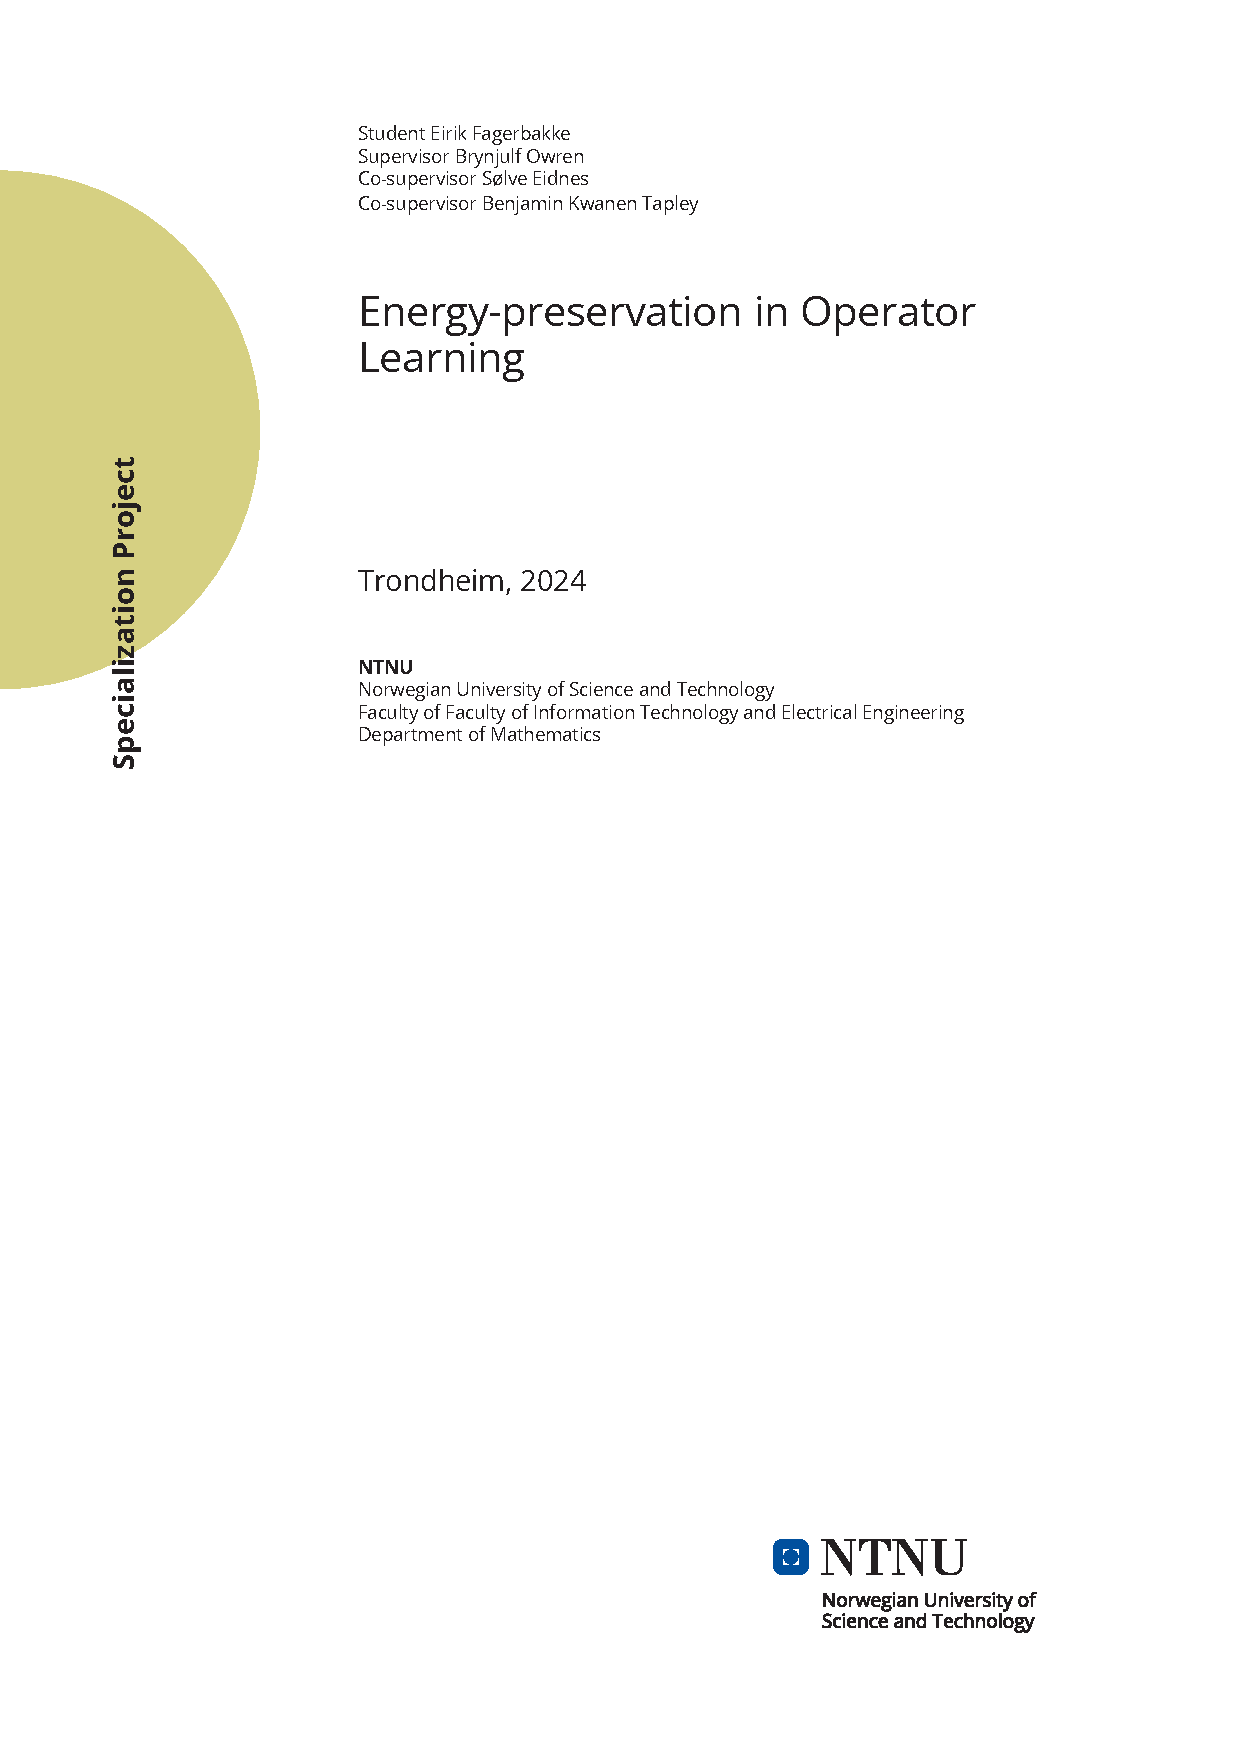
\includepdf[pages=-]{titlepage.pdf}

%----------------------------------------------------------------------------------------
%	BOOK INFORMATION
%----------------------------------------------------------------------------------------

\titlehead{Specialization Project}
\title[Energy-preservation in Operator Learning]{Energy-preservation in Operator Learning}
\author[EF]{Eirik Fagerbakke}
\date{\today}

%----------------------------------------------------------------------------------------

\frontmatter % Denotes the start of the pre-document content, uses roman numerals

%----------------------------------------------------------------------------------------
%	PREFACE
%----------------------------------------------------------------------------------------

%\chapter*{Preface}

%----------------------------------------------------------------------------------------
%	TABLE OF CONTENTS & LIST OF FIGURES/TABLES
%----------------------------------------------------------------------------------------

\begingroup % Local scope for the following commands

% Define the style for the TOC, LOF, and LOT
%\setstretch{1} % Uncomment to modify line spacing in the ToC
%\hypersetup{linkcolor=blue} % Uncomment to set the colour of links in the ToC
\setlength{\textheight}{230\vscale} % Manually adjust the height of the ToC pages

% Turn on compatibility mode for the etoc package
\etocstandarddisplaystyle % "toc display" as if etoc was not loaded
\etocstandardlines % "toc lines as if etoc was not loaded

\tableofcontents % Output the table of contents

\listoffigures % Output the list of figures

% Comment both of the following lines to have the LOF and the LOT on different pages
\let\cleardoublepage\bigskip
\let\clearpage\bigskip

\listoftables % Output the list of tables

\endgroup

%----------------------------------------------------------------------------------------
%	MAIN BODY
%----------------------------------------------------------------------------------------

\mainmatter % Denotes the start of the main document content, resets page numbering and uses arabic numbers
\setchapterstyle{kao} % Choose the default chapter heading style

%----------------------------------------------------------------------------------------
%	INTRODUCTION
%----------------------------------------------------------------------------------------

\newgeometry{
    top=25mm,             % height of the top margin
    bottom=30mm,          % height of the bottom margin
    inner=24.8mm,           % width of the inner margin
    textwidth=117mm,        % width of the text
    marginparsep=8.2mm,     % width between text and margin
    marginparwidth=40mm,  % width of the margin
}%
% !TeX root = ..\main.tex
\chapter{Introduction}

\section{Motivation}

The use of neural networks to learn functions has in general seen a lot of success, where we learn a mapping between 
finite-dimensional Euclidean spaces. A different and more recent approach is to learn operators, and has garnered a lot of attention \sidecite{kovachkiOperatorLearningAlgorithms2024}. 
The first architecture with the goal of learning \textit{operators}, rather than functions, was introduced in 2019 \sidecite{luDeepONetLearningNonlinear2021,luComprehensiveFairComparison2022}.
This was named the \textit{DeepONet}, and allowed for mapping from a discretized function to an infinite-dimensional function space.
Since then, a plethora of other architectures and extensions have been proposed \cite{caoLNOLaplaceNeural2023,seidmanNOMADNonlinearManifold2022,xiongKoopmanNeuralOperator2024,wangImprovedArchitecturesTraining2022a,lanthalerOperatorLearningPCANet2023,prasthoferVariableInputDeepOperator2022}. 
Perhaps most notably, a family of methods dubbed \textit{Neural Operators} were introduced in \cite{kovachkiNeuralOperatorLearning2024}. Of these, the 
method known as the \textit{Fourier Neural Operator} (FNO) introduced in \sidecite{liFourierNeuralOperator2021,kovachkiNeuralOperatorLearning2024} has seen a lot of success.

The use of operator learning allows us to learn the solution operator of a partial differential equation (PDE) directly 
from data. It is previously known that methods informed about the underlying physics of the problem, so-called Physics-Informed Neural Networks (PINNs), can outperform purely data-driven methods \sidecite{raissiPhysicsinformedNeuralNetworks2019,karniadakisPhysicsinformedMachineLearning2021}.
This has also been explored for Neural Operators in \sidecite{liPhysicsInformedNeuralOperator2023} and for the DeepONet in \sidecite{wangLearningSolutionOperator2021}.
These approaches do however require that we know the underlying PDE, or at least its general form, which is not always the case.

The \textit{Hamiltonian Neural Networks} (HNN) \sidecite{greydanusHamiltonianNeuralNetworks2019} 
and \textit{Lagrangian Neural Networks} (LNN) \sidecite{cranmerLagrangianNeuralNetworks2020} instead work by strictly imposing the Hamiltonian or Lagrangian structure of the problem, respectively, to learn an ordinary differential equation (ODE).
These approaches have been further explored for Pseudo-Hamiltonian systems in \sidecite{eidnesPseudoHamiltonianNeuralNetworks2023}, and were then extended to partial differential equations (PDEs) in \sidecite{eidnesPseudoHamiltonianNeuralNetworks2024}.
A similar approach to the HNN, but in the context of Hamiltonian PDEs and operator learning, were also proposed in \sidecite{tanakaNeuralOperatorsMeet2024}. This paper introduces the \textit{Energy-consistent Neural Operator} (ENO), where they apply an energy-penalty to the loss function, similar to a PINN.
The paper does however use the more traditional multilayer perceptron (MLP) architecture, instead of the operator learning methods previously mentioned.

This project will focus on comparing different DeepONet and FNO architectures for solving Hamiltonian PDEs,
and will in particular build on the work of \cite{tanakaNeuralOperatorsMeet2024} by introducing a
\textit{Hamiltonian Operator Network} (HON). In this architecture, we will investigate the implementation and use of the different operator learning frameworks previously mentioned.
We will also investigate imposing the Hamiltonian structure through a penalty term as in the ENO approach, or directly
through the architecture, akin to the HNN approach.

Our proposed HON architecture allows for using the existing operator learning architectures, while also imposing a Hamiltonian structure on the learned operator, with no previous knowledge of the underlying PDE.
The learned operator will then enjoy the benefits of both the operator learning architecture and the learned Hamiltonian structure. Specifically, we will then achieve networks that are universal approximators of operators.
The use of such an architecture also poses the problem of how one should compute the derivatives of the learned operator, which is not trivial in general, and is something we have had to address for the networks discussed in this project.

\section{Problem setting}

Following similar notation as \sidecite{tanakaNeuralOperatorsMeet2024} and \sidecite{kovachkiNeuralOperatorLearning2024}, we want to learn an approximation to an operator \(\mathcal{S}\), which maps from the input function space \(\mathcal{A}\) to the output function space \(\mathcal{U}\).
\(\mathcal{A}\) and \(\mathcal{U}\) are assumed to be Banach spaces. \(\mathcal{A}\) consists of functions defined on the bounded spatial domain \(\mathcal{X} \subset \mathbb{R}^d \), and \(\mathcal{U}\) consists of functions defined on the spatial-temporal domain \(\mathcal{Y} = \mathcal{T} \times \mathcal{X} \subset \mathbb{R}^{d+1}\). 

The input function is denoted by \(a : \mathcal{X} \to \mathbb{R}^{d_a}\), with \(a \in \mathcal{A}\). It may in general correspond to the initial condition, a forcing term or a coefficient in the PDE. In this project, \(a\) shall refer to the initial condition of the PDE. 
The output function is denoted by \(u: \mathcal{Y} \to \mathbb{R}^{d_u}\), with \(u = \mathcal{S}[a]  \in \mathcal{U}\). \(\mathcal{S}\) is then the solution operator for the PDE.

We assume that we have some observations \(\{a^{(i)}, u^{(i)}\}_{i=1}^N\) of the input-output pairs, where \(a^{(i)} \sim \mu\) are assumed to be i.i.d. samples drawn from some probability measure \(\mu\) supported on \(\mathcal{A}\), and \(u^{(i)} = \mathcal{S}[a^{(i)}]\) are the corresponding outputs.

Our goal is then to learn a neural network that approximates this operator, i.e. \(\mathcal{S}_\theta[a] \approx \mathcal{S}[a]\), where \(\theta \in \mathbb{R}^q\) are the parameters of the neural network.

We are further going to consider PDEs which have an energy functional, and we want the predictions of the neural network to preserve an approximation to the energy (or more precisely the \textit{Hamiltonian}) of the governing PDE, which we discuss in \cref{sec:HINO_theory}.

A summary of the notation introduced here, and in other sections of the project, can be found in \cref{tab:notation}.
\pagelayout{margin} % Restore margins

%----------------------------------------------------------------------------------------
%	THEORY
%----------------------------------------------------------------------------------------

% !TeX root = ..\main.tex
\chapter{Background on DeepONets and Neural Operators}

\subsection{DeepONet}

\subsubsection{The Vanilla DeepONet}
In \sidecite{luDeepONetLearningNonlinear2021}, the authors introduce the DeepONet. 
The vanilla DeepONet is a network that takes a discretized function, $a$, as input (evaluated at \(p\) fixed "sensors"). 
It also takes a query point $y \in \mathcal{Y}$, which is where we want the output to be evaluated in the output domain.
We then want the network to learn an operator $\mathcal{S}$, such that $\mathcal{S}[a](y) = u(y)$. 
It is important to note that the query points $y$ are independent of the placements of the fixed sensors. 
This then leads to a network architecture that maps from a finite-dimensional space to an infinite-dimensional one.

The motivation behind the network architecture stems from the Universal approximation theorem 
by Chen \& Chen \sidecite{tianpingchenUniversalApproximationNonlinear1995,luDeepONetLearningNonlinear2021}, where they originally 
consider a shallow neural network. The authors of \sidecite{luDeepONetLearningNonlinear2021} then build a deep structure based on this. The theorem
is reiterated below, with notation that matches ours:

\begin{theorem}[Universal approximation theorem for operators]
    \hfill\\
    Suppose that $\sigma$ is a continuous nonpolynomial function, 
    $X$ is a Banach Space, $\mathcal{X} \subset X, \mathcal{Y} \subset \mathbb{R}^{d+1}$ are two compact sets,
    $\mathcal{A}$ is a compact set in $C\left(\mathcal{X}\right)$, $\mathcal{S}$ is a nonlinear continuous operator, 
    which maps $\mathcal{A}$ into $C\left(\mathcal{Y}\right)$. Then for any $\epsilon>0$, there are positive integers $n, p, m$, 
    constants $c_i^k, \xi_{i j}^k, \theta_i^k, \zeta_k \in \mathbb{R}, w_k \in \mathbb{R}^{d+1}, x_j \in K_1$, 
    $i=1, \ldots, n$, $k=1, \ldots, p$, $j=1, \ldots, m$, such that
    
    \begin{equation}
        \left|\mathcal{S}[a](y)-\sum_{k=1}^p 
        \underbrace{\sum_{i=1}^n c_i^k \sigma\left(\sum_{j=1}^m \xi_{i j}^k a(x_j)+\theta_i^k\right)}_{\text {branch }} 
        \underbrace{\sigma\left(w_k \cdot y+\zeta_k\right)}_{\text {trunk }}\right|<\epsilon
    \end{equation}
    
    holds for all $a \in \mathcal{A}$ and $y \in \mathcal{Y}$.
    \label{thm:universal_approximation_thm}
\end{theorem}

Based on \cref{thm:universal_approximation_thm}, the DeepONet is split into two parts: the \textit{trunk} and the \textit{branch} nets. 
The trunk net takes the query point $y$ as input, and the branch net takes the discretized function $a$ as input.
The outputs of the branch and trunk nets result in two \(p\)-dimensional vectors, which are then combined in a 
linear fashion via a dot product. It should be noted that the DeepONet is origianlly defined for scalar-valued functions, but can
be generalized to vector-valued functions as well, see for instance \sidecite{wangLongtimeIntegrationParametric2021}.

The authors discuss some slightly varying architectures. 
One option they suggest uses a "stacked DeepONet", meaning that we have \(p\) different branch networks, each one producing one element in the 
branch net vector.
Another way is to use the "unstacked DeepONet", where we use only a single network to produce all the \(p\) branch elements directly.
Although \cref{thm:universal_approximation_thm} does not include a final bias term, the authors also discuss the possibility of 
adding a bias to the final output of the DeepONet, to allow for a more expressive model.
In this project, we have chosen to use the unstacked DeepONet with a bias, and we will be referring to this as the "Vanilla DeepONet".
The predictions can then be written as

\begin{equation}
    \mathcal{S}_\theta[a](y) = \sum_{i=1}^p b_k(a) t_k(y) + b_0,
    \label{eq:DeepONet_prediction}
\end{equation}

where $b_k(a)$ are the branch net outputs, $t_k(y)$ are the trunk net outputs, and $b_0$ is the bias term.
The branch and trunk nets can in general be parametrized by any neural network architecture, but we have chosen to use MLPs for both in this project.

The general DeepONet architecture is illustrated in \cref{fig:DeepONet}.

\begin{figure}[h!]
    \centering
    \includesvg{DeepONet}
    \caption[DeepONet architecture]{DeepONet architecture.}
    \label{fig:DeepONet}
\end{figure}

\subsubsection{Evaluation of the DeepONet}

The DeepONets are evaluated on single coordinates, so in order to get a prediction for the whole domain, we have to evaluate the model multiple times. 
This can be done by for instance utilizing \texttt{vmap} in \texttt{JAX}, which vectorizes a function automatically. However, as discussed in \sidecite{luComprehensiveFairComparison2022}, we can
make the computation even more efficient by re-using predictions from the branch and trunk nets. If we have a single input function which we want to evaluate at multiple points,
we may evaluate the branch net once only, and combine it with the predictions of the trunk net by a matrix multiplication. The same holds for when we have multiple input functions and a single query point,
or when we have multiple input functions and multiple query points.

\subsubsection{DeepONet extensions}

There have been made several extensions to the vanilla DeepONet architecture. One noteable example includes the POD-DeepONet, 
introduced in \sidecite{luComprehensiveFairComparison2022}, where some of the authors of the original DeepONet paper 
discuss an enhancement of their original architecture. 
The POD-DeepONet uses a pre-computed POD-basis, denoted by \(\{\phi_k\}\), generated from the training data, in place of the trunk net.
Instead of learning the basis for the query points, these are now pre-computed, and the network only learns the branch net parameters.
The output can then be written as 
\begin{equation}
    \mathcal{S}_\theta[a](y) = \sum_{i=1}^p b_k(a) \phi_k(y) + \phi_0(y).
    \label{eq:POD-DeepONet}
\end{equation}
With the improved results seen in \cite{luComprehensiveFairComparison2022}, this could be an interesting extension to explore. However, we have chosen
to focus on the original DeepONet architecture as it is more general and expressive.

One criticism of the DeepONet, is that it is not able to take input functions at any point; the number of "sensors" and their placement remains fixed.
A possible extension which allows for variable input in the branch-net has been discussed in \sidecite{prasthoferVariableInputDeepOperator2022, hoopCostAccuracyTradeOperatorLearning2022}, 
where they develop an enhanced architecture which allows for a varying number and placement of sensors. 
In this project, we have however chosen to generate the data such that the input functions are evaluated at a fixed set of sensors, as originally proposed in \cite{luDeepONetLearningNonlinear2021}.

Lastly, we note the "Modified DeepONet", introduced in \sidecite{wangImprovedArchitecturesTraining2022a}. 
The authors of \cite{wangImprovedArchitecturesTraining2022a} argue that their
proposed architecture should help the inputs propagate throughout the network, and their modification empirically led to more 
accurate predictions in all examples discussed in \cite{wangImprovedArchitecturesTraining2022a}.
In addition, another criticism of the DeepONet is that the input function and the query point is combined in a linear fashion, which leads to a linear 
approximation of the \textit{operator} that we want to learn \sidecite{kovachkiNeuralOperatorLearning2024}.
The Modified DeepONet circumvents this by creating encoders for both the branch and trunk nets, which are combined throughout
the networks. The predictions are now written as

\begin{align*}
    B_E &= \sigma(W_a a + b_a), \qquad\qquad\qquad\qquad T_E = \sigma(W_yy + b_y), \\
    B^{(1)} &= \sigma(W_a^{(1)} a + b_a^{(1)}), \qquad\qquad\qquad T^{(1)} = \sigma(W_y^{(1)}T + b_y^{(1)}), \\
    B^{(l+1)} &= (1- \sigma(W_a^{(l)}B^{(l)}+b_a^{(l)})) \odot B_E + \sigma(W_y^{(l)}T^{(l)}+b_y^{(l)}) \odot T_E\\
    T^{(l+1)} &= (1- \sigma(W_y^{(l)}T^{(l)}+b_y^{(l)})) \odot B_E + \sigma(W_a^{(l)}T^{(l)}+b_a^{(l)}) \odot T_E\\
    B^{(L)} &= \sigma(W_a^{(L)} B^{(L-1)} + b_u^{(L)}), \qquad\qquad T^{(L)} = \sigma(W_y^{(L)}T^{(L-1)} + b_y^{(L-1)}), \\
    \mathcal{S}_\theta[a](y) &= \langle B^{(L)}, T^{(L)}\rangle + b_0,
\end{align*}

where \(B_E\) and \(T_E\) are the encoders for the branch and trunk nets, respectively, and \(\sigma\) is the activation function.
The \(W\) and \(b\) are the weights and biases of the networks, and the \(\odot\) denotes element-wise multiplication.
\(B^{(l)}\) and \(T^{(l)}\) are the outputs of the branch and trunk nets at layer \(l\), respectively.
Finally, we also allow for a final bias term, \(b_0\), to be added to the output.

This network architecture is illustrated in \cref{fig:Modified_DeepONet}.

\begin{figure}[h!]
    \centering
    \includesvg{Modified_DeepONet}
    \caption[Modified DeepONet architecture]{Modified DeepONet architecture, based on diagram in \cite{wangImprovedArchitecturesTraining2022a}.}
    \label{fig:Modified_DeepONet}
\end{figure}
 
Motivated by the results seen in \cite{wangImprovedArchitecturesTraining2022a}, we have chosen to also implement and compare this modified architecture agains the vanilla DeepONet.

\subsection{Neural Operators}

A different and more recent approach to operator learning is discussed in \sidecite{kovachkiNeuralOperatorLearning2024}.
While the (vanilla) DeepONets take discretized functions as inputs, and therefore technically map from a finite dimensional space to a 
function space, the Neural Operators are defined as mappings between function spaces. In this section, we will start by quickly reiterating
the building blocks of a general Neural Operator, as they are defined in \cite{kovachkiNeuralOperatorLearning2024}.

The network architechture can be seen as an extension of MLPs to function spaces. Instead of the traditional fully-connected layers, 
the networks employ "integral kernel operators", which similarly are meant to capture the global features through an integral over the domain:

\begin{definition}[Integral Kernel Operators]
    \begin{equation}
        (\mathcal{K}v_l)(z) = \int_D \kappa^{(l)}(z,\bar{z}) v_l(\bar{z}) \, d \nu_l(\bar{z}). 
        \labdef{kernel_operator}
    \end{equation}
\end{definition}

Here, \(v_l\) is the input function, \(\kappa^{(l)}\) is the kernel function, and \(d \nu_l\) is the measure over the domain \(D\).
We write \(z\) to denote the inputs to the functions, as the input to the model can vary. Later, we will investigate how to handle the time dimension, and
\(z\) may represent either only a spatial coordinate, \(z=x\), or it may refer to points in the spatial-temporal domain \(z=y=(x,t)\).

The paper also defines two other alternative kernel integral operator definitions, but we will use the basic form defined in \refdef{kernel_operator} with \( d \nu_l\) being the Lebesgue measure.
In addition to the integral kernel operators, the article also defines three additional pointwise operators.

\begin{enumerate}
    \item A lifting layer, \(\mathcal{P}\), which lifts the input function's codimension: \(\{a : D \to \mathbb{R}^{d_a}\} \mapsto \{v_0 : D \to \mathbb{R}^{d_{v_0}}\}\).
    \item Linear layers, \(\mathcal{W}_l\), which are the local transformations of each Neural Operator layer.
    \item A projection layer, \(\mathcal{Q}\), which maps back to the desired codimension: \(\{v_L : D' \to \mathbb{R}^{d_{v_L}}\} \mapsto \{u : D' \to \mathbb{R}^{d_u}\}\).
\end{enumerate}

It is also usual to incorporate bias terms in neural networks. In the context of neural operators, these are included as bias \textit{functions}, \(b_l(z)\).

This all comes together as 

\begin{definition}[Neural Operator \(\mathcal{S}_\theta\)]
    \begin{equation}
        \mathcal{S}_\theta =  \mathcal{Q} \circ \sigma_L (\mathcal{W}_L + \mathcal{K}_L + b_L) \circ \dots \circ \sigma_1 (\mathcal{W}_1 + \mathcal{K}_1 + b_1)\circ \mathcal{P}
        \label{eq:neural_operator}
    \end{equation}
\end{definition}

where \(\sigma_l\) denotes non-linear activation functions. A visualization of the Neural Operator architecture can be seen in \cref{fig:Neural_Operator}.

\begin{figure}[h!]
    \centering
    \includesvg{Neural_Operator}
    \caption[Neural Operator architecture]{Neural Operator architecture.}
    \label{fig:Neural_Operator}
\end{figure}


The methods are then implemented by using discretized versions of the operators and functions.
The local linear operators, \(\mathcal{W}_l\), are usually implemented as either \(1\times1\) convolutions or by the multiplication with a matrix \(W_l \in \mathbb{R}^{d_{v_{l}} \times d_{v_{l-1}}}\) \sidecite{kossaifiLibraryLearningNeural2024,luComprehensiveFairComparison2022}.
In this project, we have chosen to do the latter.

The bias functions are usually implemented simply as a learnable vector, \(b_l \in \mathbb{R}^{d_{v_l}}\) \sidecite{kossaifiLibraryLearningNeural2024}. This means that the we have a constant function which does not depend on \(z\). 
Other alternatives could be to parametrize it by a shallow neural network or with coefficients multiplied with a fixed basis.

Lastly, \cite{kovachkiNeuralOperatorLearning2024} 
define three different suggestions for discretized integral kernel operators: the "Graph Neural Operator" (GNO), the "Low-rank Neural Operator" (LNO) and the 
"Fourier Neural Operator" (FNO). 
Especially the FNO has garnered a lot of attention for its good results on PDEs and its 
efficiency by utilizing the fast Fourier transform (FFT). This is done by assuming a kernel of the form \(\kappa(z,\bar{z})=\kappa(z-\bar{z})\) 
and using the convolution theorem of the Fourier Transform \cite{kovachkiNeuralOperatorLearning2024}:

\begin{equation}
    \mathcal{K}(v)(z) 
    = \int_D \kappa(z-\bar{z} ) v(\bar{z} ) \, d\bar{z} 
    = \mathcal{F}^{-1} (\mathcal{F}(\kappa) \mathcal{F}(v))(z)
    = \mathcal{F}^{-1} (R \mathcal{F}(v))(z),
\end{equation}

where \(\mathcal{F}(\kappa)\) is parametrized directly by a matrix \(R\) of learnable weights.
The Fourier transform and its inverse are then replaced by the FFT and the inverse fast Fourier transform (IFFT), leading to an efficient approximation of the integral kernel operator \sidecite{kovachkiNeuralOperatorLearning2024}.

In this project, we have decided to limit our exploration of the Neural Operators to the FNO.

\subsubsection{Appending the grid to the input}\label{sec:appending_grid}

From the definition of the Neural Operators, we see that there is no need to give the grid that the input function is evaluated on as input to the network.
This is however often done in practice by appending the grid to the input function, and usually gives better results \sidecite{kovachkiNeuralOperatorLearning2024,luComprehensiveFairComparison2022}.
This essentially means that we now view our input function as a vector-valued function, which also outputs the grid points.
If we for instance add the spatial coordinates to our input function \(a : x \mapsto a(x)\), we can instead evaluate \(v : x \mapsto (x, a(x))\).
We do this for all of the FNO-based models considered.

\subsubsection{Incorporating the time dimension in the FNO}

As was also discussed in \sidecite{luComprehensiveFairComparison2022}, the FNO requires \(D\) and \(D'\) to be from the same domain.
Since we are trying to learn the mapping from an initial condition, at time \(t=0\), to the solution for \(t \in [0, T]\), this has to be accounted for.
In our problem setting, we have \(D = \mathcal{X}\) and \(D' = \mathcal{Y} = \mathcal{X} \times \mathcal{T}\).
We present three possible solutions:

\textbf{Method 1: Timestepping.} We learn an operator \(\tilde{\mathcal{S}_\theta} : u(x, t) \mapsto u(x,t + \Delta t)\),
where \(\Delta t\) is a fixed step size. We can then iteratively apply this operator to get predictions for discrete time points.
In order to make this method continuous in time, we will have to interpolate between the discrete time points.
This method performs the FFT in space only, and will be referred to as "\texttt{FNOTimestepping}". This method was also mentioned 
in \sidecite{kovachkiNeuralOperatorLearning2024, luComprehensiveFairComparison2022}.

\textbf{Method 2: Extending the domain.} We extend the domain of our initial condition to \(\mathcal{Y}\), by viewing it as a function that is constant in time, \(a(x,t)=a(x)\).
The integral kernel operator will then act on the whole spatial-temporal domain, meaning that we need to perform the 2D FFT.
This method will therefore be referred to as "\texttt{FNO2d}". The method was also discussed in \sidecite{luComprehensiveFairComparison2022}.

\textbf{Method 3: Query points in time.} We introduce here a third method that, as far as we know, has not been discussed in the literature before. In this method, we also view \(a\) as a function on 
\(\mathcal{Y}\) that is constant in time, but we only learn the spatial mapping. 
The time coordinate then essentially acts as a "query point", telling us where in the temporal output domain we want the prediction.
With this method, it is necessary to append the time coordinate to the input function, as discussed in \cref{sec:appending_grid}, to allow the network to differentiate between different time points.
The input function is then \(v : x \mapsto (a(x), t)\), where \(t\) is the time point we want to evaluate the solution at.
We can also add the spatial grid points to the input as before.
This method will be referred to as "\texttt{FNO1d}".

\subsection{A brief comparison between the different approaches}

Both the DeepONet and the Neural Operators are shown to be universal approximators of operators. 
Specifically, the Neural Operators are shown to uniformly approximate any continuous operator defined on a compact set of Banach spaces in 
\sidecite{kovachkiNeuralOperatorLearning2024}, and from before we have the universal approximation theorem for the DeepONet seen in \cref{thm:universal_approximation_thm}.
This property does not apply to the traditional neural networks \cite{kovachkiNeuralOperatorLearning2024}, and is a big motivation for using DeepONets or Neural Operators for operator learning.
Even though the DeepONet is a universal approximatior, it combines the branch and trunk nets in a linear fashion, leading to a linear approximation of the operator . The Neural Operators, on the other hand, are non-linear approximations to the operator, which in general should allow for a more expressive model \cite{kovachkiNeuralOperatorLearning2024}.

The Neural Operators do however encompass a property that sets them apart from the DeepONets. They are \textit{discretization-invariant}, a property proposed in \cite{kovachkiNeuralOperatorLearning2024}. 
According to \cite{kovachkiNeuralOperatorLearning2024}, they are also the only known class of methods to encompass this property.
A discretization-invariant model is defined by the following properties \cite{kovachkiNeuralOperatorLearning2024}:

\begin{definition}[Discretization-invariant operator]
    \hfill\\
    A discretization-invariant model satisfies the following properties:
    \begin{enumerate}
        \item acts on any discretization of the input function, i.e. accepts any set of points in the input domain,  
        \item can be evaluated at any point of the output domain,  
        \item converges to a continuum operator as the discretization is refined.
    \end{enumerate}
    \labdef{discretization_invariant_operator}
\end{definition}

In comparison, the vanilla DeepONet fulfills the second property, but it does not fulfill the first or third. 
The Vanilla DeepONet cannot take the input function at any point, as the branch net limits the input to the fixed "sensors".
As discussed previously, there have however been made some generalizations which circumvent this \sidecite{hoopCostAccuracyTradeOperatorLearning2022,kovachkiNeuralOperatorLearning2024,prasthoferVariableInputDeepOperator2022}.

The DeepONet does not fulfill the third property, as its predictions does not converge with a finer grid size. Since the network takes query points, rather than a grid, the model's prediction at the same query point will not change with the mesh size.
This contrasts with the Neural Operators, which take values on a grid, and the predictions converge as the step size decreases \cite{kovachkiNeuralOperatorLearning2024}.

Another big difference between the DeepONet and the Neural Operators, is in the inputs and outputs of the methods. As stated previously, 
the DeepONet takes a query point \(y\) from the output domain and predicts \(\mathcal{S}_\theta[a](y) \approx u(y)\big|_a\). The inputs and outputs of the DeepONet (and the "Modified" variant) can then be written as

\begin{equation}
    \text{DeepONet} : 
    \underbrace{\mathbb{R}^{N}}_{\substack{\text{branch input,} \\ \text{\(a(x)\) at \(N\) sensors.}}}
    \times 
    \underbrace{\mathbb{R}^{d+1}}_{\substack{\text{trunk input,} \\ \text{query point \(y\).}}} 
    \to 
    \underbrace{\mathbb{R}}_{\substack{\text{prediction,} \\ \text{\(u\) at \(y\)}}}.
\end{equation}

The Neural Operators do not take query points, but rather directly compute the prediction at all given input points, 
\(\mathcal{S}_\theta[a] \approx u\). The number of "input points" depends on the method we use. Below we list the mappings for the different methods we have considered:
\begin{equation}
    \text{FNO2d} : 
    \underbrace{\mathbb{R}^{N_x \times N_t}}_{\substack{\text{initial condition,} \\ \text{\(a(x,t)=a(x)\)}}}
    \to 
    \underbrace{\mathbb{R}^{N_x \times N_t}}_{\substack{\text{prediction,} \\ \text{\(u(x,t)\)}}}
\end{equation}

\begin{equation}
    \text{FNO1d} : 
    \underbrace{\mathbb{R}^{N_x}}_{\substack{\text{initial condition,} \\ \text{\(a(x)\)}}} \times \underbrace{\mathbb{R}}_{\substack{\text{time point \(t^*\)}}}
    \to 
    \underbrace{\mathbb{R}^{N_x}}_{\substack{\text{prediction,} \\ \text{\(u(x,t^*)\)}}}
\end{equation}

\begin{equation}
    \text{FNOTimeStepping} : 
    \underbrace{\mathbb{R}^{N_x}}_{\substack{\text{input function,} \\ \text{\(u(x,t^*)\)}}} 
    \to 
    \underbrace{\mathbb{R}^{N_x}}_{\substack{\text{prediction,} \\ \text{\(u(x,t^*+\Delta t)\)}}}
\end{equation}

This difference in input will also affect both the loss function and how we can compute derivatives. 
For the DeepONets we are able to sample the query points randomly, so we can then compute the loss function by evaluating the network at these points only.
This also applies to the FNO1d approach, where we can sample the time points randomly. The same holds for the derivatives, where we for the DeepONets can compute them directly at the query points only.
The query points of the DeepONet therefore makes it more flexible in general. To evaluate on a grid, we simply vectorize over the grid points.
We will discuss both the loss function used, and the computation of the derivatives, in more detail in the following sections.

\chapter{Operator Learning for Hamiltonian PDEs} \label{sec:HINO_theory}

\subsection{Hamiltonian PDEs}

A Hamiltonian PDE can be written on the form 
\begin{equation}
    u_t = \mathcal{G} \frac{\delta \mathcal{H}}{\delta u}
    \label{eq:hamiltonian_pde}
\end{equation}

where \(\mathcal{G}\) is a Hamiltonian operator, \(\mathcal{H} : \mathcal{U} \to \mathbb{R}\) is the Hamiltonian functional of the system, and \(\frac{\delta \mathcal{H}}{\delta u}\) is the variational derivative \cite{leimkuhlerSimulatingHamiltonianDynamics2005, olverApplicationsLieGroups1986}.
In order for \(\mathcal{G}\) to be a Hamiltonian operator, it needs to be a constant linear operator, and it also has to satisfy two conditions on its Poisson bracket. These are the conditions of skew-symmetry and the Jacobi identity. We skip the details here, but refer the reader to \cite{olverApplicationsLieGroups1986}.
We will in our project assume that \(\mathcal{G}=-\partial_x\), which does indeed satisfy the conditions of a Hamiltonian operator.
The Hamiltonian functional can furthermore be written as \[\mathcal{H} = \int_{\mathcal{X}} F(x; u, u_x, u_{xx}, \ldots) dx,\] where \(F : \mathcal{U} \to \mathbb{R}\) is the \textit{energy density function} \cite{olverApplicationsLieGroups1986,tanakaNeuralOperatorsMeet2024,celledoniPreservingEnergyResp2012}.

We can then follow the formula in \sidecite{tanakaNeuralOperatorsMeet2024,  olverApplicationsLieGroups1986, celledoniPreservingEnergyResp2012}, which states that 

\begin{equation}
    \frac{\delta \mathcal{H}[\vect{u}]}{\delta u_m} = \frac{\partial F}{\partial u_m}  - \sum_{d=1}^{D}\left[ \frac{\partial}{\partial x_d} \frac{\partial F}{\partial u_{m,d}} \right] + \ldots
    \label{eq:variational_derivative}
\end{equation}

where \(u_m\) is the \(m\)-th component of \(\vect{u}\), \(x_m\) is the \(m\)-th component of the spatial coordinate, and \(F\) is the energy density function of the Hamiltonian. \(u_{m,d}\) refers to the derivative of \(u_m\) with respect to \(x_d\).

\subsection{The Energy-consistent Neural Operator}

There are now two main approaches to satisfying the constraint of \cref{eq:hamiltonian_pde} in our network: hard or soft constraints.
The easiest of the two to employ, is usually the soft constraints, where we add a term to the loss function that we wish to minimize.
This term then pushes the network towards satisfying the constraints, but does not necessarily guarantee that they are satisfied.
Hard constraints, on the other hand, enforce the constraints directly, thereby ensuring that they are exactly satisfied \sidecite{karniadakisPhysicsinformedMachineLearning2021}.

In \sidecite{tanakaNeuralOperatorsMeet2024}, the authors introduced the "Energy-consistent Neural Operator" (ENO).
This network consists first of an MLP, which takes a stacked vector of a discretized initial condition \(a(x)\) and a query point \((x,t)\) as input. It then outputs an approximation to \(\mathcal{S}[a](x,t)=u(x,t)\).
They then compute derivatives \(u_t\) and \(u_x, u_{xx}, \ldots\) by automatic differentiation. These values are then the inputs to another neural network, \(F_\phi\), which parametrizes the energy density function \(F\).
They then proceed by computing the right-hand side of \cref{eq:hamiltonian_pde}, again through automatic differentiation, by using the variational derivative of the Hamiltonian, as seen in \cref{eq:variational_derivative}. 

The ENO is "informed" about the Hamiltonian structure of the PDE, in the sense that \(\dot{u}_m^\theta\) and \(\mathcal{G} \frac{\delta \mathcal{H}_\phi[\vect{u}^\theta]}{\delta u_m^\theta}\) are 
pushed to equality by adding a penalty term to the loss function. This is a "soft constraint", as the network is not 
guaranteed to satisfy \cref{eq:hamiltonian_pde} exactly.
This follows the same general strategy as we see in the well-known physics-informed neural networks (PINNs) \sidecite{raissiPhysicsinformedNeuralNetworks2019}.

It should also be noted that the ENO, as it was introduced in \cite{tanakaNeuralOperatorsMeet2024}, does not use the DeepONet or a Neural Operator in its approach, but rather an MLP.
They do mention the DeepONet and FNO, but as we shall see, the inclusion of the FNO in the architectur is in particular not straightforward.
The MLP is not a universal approximator of operators, and is not discretization-inveriant.
We therefore wish to investigate how we can implement the architecture with the use of the DeepONets and the FNOs, and compare how well these perform, in addition to investigating the use of a hard constraint.

\subsection{The Hamiltonian Operator Network}

We now propose an extension to the ENO, which uses the DeepONet or the FNO as the operator network, in addition to a hard-constrained approach.
Rather than using the predictions from the operator network, we could instead impose \(\dot{u}_m^\theta = \mathcal{G} \frac{\delta \mathcal{H}_\phi[\vect{u}^\theta]}{\delta u_m^\theta}\) directly.
We then have a network which predicts temporal derivatives that are guaranteed to preserve the approximated Hamiltonian functional, \(\mathcal{H}_\phi = \int_{\mathcal{X}}F_\phi(u^\theta, u_x^\theta, \ldots) dx\). 
To obtain the final predictions for \(u\), we can then integrate \(\dot{u}_m^\theta\) in time:

\begin{equation}
    u_m^\theta(x,t) = u_m^\theta(x,0) + \int_0^t \mathcal{G} \frac{\delta \mathcal{H}_\phi[\vect{u}^\theta]}{\delta u_m^\theta} d\bar{t}.
    \label{eq:hard_constrained_approach}
\end{equation}

This approach follows a similar structure as the one proposed in \cite{greydanusHamiltonianNeuralNetworks2019} for ODEs,
but in this case for PDEs used with the Operator Learning framework.

As we cannot find the exact antiderivative to \(\mathcal{G} \frac{\delta \mathcal{H}_\phi[\vect{u}^\theta]}{\delta u_m^\theta}\), we will have to approximate it by a numerical method.
To this end, we here list three possible methods to approximate the antiderivative:

\begin{enumerate}
    \item \textbf{Cumulative integration:} This is the simplest method where we first predict values for the integrand on grid points. 
    We then cumulatively integrate, using for instance Simpson's rule or the trapezoid rule. This can easily be done with \texttt{cumulative\_trapezoid} or \texttt{cumulative\_simpson} functions,
    found in libraries such as \texttt{scipy} or \texttt{quadax}. This approach does however introduce discretization errors which accumulate over time, and is therefore not the most suitable approach.
    \item \textbf{Exact antiderivative of interpolated function:} With this method, we first predict the integrand on grid points, and then interpolate the function.
    We can then find the exact antiderivative of the interpolated function, and evaluate it at the desired time points. This is easily done by leveraging functions such as \texttt{interp1d} in \texttt{scipy} or
    the \texttt{interpax} library. If we use sufficiently many points, and use a suitable interpolation method, this should give better results than the cumulative integration as we avoid errors that accumulate over time.
    \item \textbf{ODE integration:} A final approach is to numerically integrate by solving the initial value problem
    \[f(u_m, t) = \mathcal{G} \frac{\delta \mathcal{H}_\phi[\vect{u}]}{\delta u_m}, \qquad u_m(x, 0) =  u_m^\theta(x,0).\]
    We should also solve this using a symplectic integrator, which will preserve a discrete version of the \textit{learned} Hamiltonian.
    Note that we have a directly integrable ODE, as we know the right-hand sides direct dependence on \(t\), and we therefore do not need to solve any implicit equations.
    This method should be the preferred one.
\end{enumerate}

\section{Computing the functional derivative}

In order to compute our model's prediction for the right-hand side of \cref{eq:hamiltonian_pde}, we need to compute the functional derivative of the Hamiltonian.


In this project, we will only consider scalar-valued functions in one spatial dimension. 
In addition, we assume that our energy density function \(F\) only depends on \(u\) and \(u_x\). The formula then simplifies to

\begin{equation}
    \frac{\delta \mathcal{H}[u]}{\delta u} = \frac{\partial F}{\partial u}  -  \frac{\partial}{\partial x} \frac{\partial F}{\partial u_x}.
    \label{eq:variational_derivative_simple}
\end{equation}

We will further assume that the operator \(\mathcal{G}\) is \(-\partial_x\). The right-hand side of \cref{eq:hamiltonian_pde} can then be written as

\begin{equation}
    \mathcal{G}\frac{\delta \mathcal{H}[u]}{\delta u} =  -\frac{\partial}{\partial x}\frac{\partial F}{\partial u}  +  \frac{\partial^2}{\partial x^2} \frac{\partial F}{\partial u_x}.
    \label{eq:rhs_pde_simplified}
\end{equation}

As \(F\) depends on \(x\) through \(u\) and \(u_x\), we can either consider total derivatives and compute them directly, or we can use the chain rule.

For the approach using the chain rule, we note that the chain rule for multivariable functions gives 

\begin{align}
    \frac{\partial}{\partial x}\frac{\partial F}{\partial u} &= \frac{\partial^2 F}{\partial u^2} u_x + \frac{\partial^2 F}{\partial u \partial u_x} u_{xx} \nonumber\\
    \frac{\partial}{\partial x}\frac{\partial F}{\partial u_x} &= \frac{\partial^2 F}{\partial u_x \partial u} u_x + \frac{\partial^2 F}{\partial u_x^2} u_{xx}.\label{eq:chain_rule1}
\end{align}

We now differentiate \cref{eq:chain_rule1} with respect to \(x\) once again, which after a thourough calculation gives

\begin{equation}
    \frac{\partial^2}{\partial x^2}\frac{\partial F}{\partial u_x}  = 
    \frac{\partial^2 F}{\partial u \partial u_x} u_{xx}
    +\frac{\partial^2 F}{\partial u_x^2} u_{xxx}
    +\frac{\partial^3 F}{\partial u_x u^2} u_x^2
    +2\frac{\partial^3 F}{\partial u_x^2 \partial u} u_x u_{xx}
    +\frac{\partial^3 F}{\partial u_x^3}  u_{xx}^2.
    \label{eq:chain_rule2}
\end{equation}

The full expression for the right-hand side of \cref{eq:hamiltonian_pde} using the multivariable chain rule is then 


\begin{align}
    \mathcal{G}\frac{\delta \mathcal{H}[u]}{\delta u} &=
    -\left(\frac{\partial^2 F}{\partial u^2} u_x + \frac{\partial^2 F}{\partial u \partial u_x} u_{xx}\right) \nonumber\\
    &+
    \frac{\partial^2 F}{\partial u \partial u_x} u_{xx}
    +\frac{\partial^2 F}{\partial u_x^2} u_{xxx}
    +\frac{\partial^3 F}{\partial u_x u^2} u_x^2
    +2\frac{\partial^3 F}{\partial u_x^2 \partial u} u_x u_{xx}
    +\frac{\partial^3 F}{\partial u_x^3}  u_{xx}^2. \nonumber\\
    \label{eq:hamiltonian_chain_rule}
\end{align}


\section{Computing spatial and temporal derivatives}

How should one go about computing spatial and temporal derivatives in the context of DeepONets and Neural Operators?
As we want the outputs of our network to satisfy \cref{eq:hamiltonian_pde}, we will need to compute
derivatives of the output \(u^\theta = \mathcal{S}_\theta[a]\) with respect to \(x\) and \(t\).

One strategy is to simply use traditional numerical methods, such as finite differences or FFT-based differentiation. 
However, this introduces discretization errors, as well as requiring sufficiently small step sizes and equidistant grids.
A more elegant and direct approach might be to utilize automatic differentiation, which can compute derivatives exactly down to floating point precision.

For the DeepONets, which take query points as input, this is possible, and we simply compute the derivatives as e.g.

\begin{equation}
    u_t^\theta = \frac{\partial \mathcal{S}_\theta}{\partial t}[a](x,t).
    \label{eq:temporal_derivative_DON}
\end{equation}

However, the situation for the Neural Operators is quite different. As discussed previously, these networks do not take query points, but 
are defined to map between function spaces directly.
Luckily, two possible solutions have been discussed in \sidecite{liPhysicsInformedNeuralOperator2023}, in addition to 
the use of traditional numerical differentiation methods. 

The solution proposed in \cite{liPhysicsInformedNeuralOperator2023} is to use the chain rule, but only for the very last layers in the neural operator.
This is not only efficient, but if we were to backpropagate through the whole network, we would in the end reach the input layer, and we do not in general know the derivative of the initial condition.

We will now illustarte how this works for the spatial derivatives by ignoring the model's dependence on \(t\). We start by writing our resulting function \(u(x)\) as it depends on the output of the previous 
layer, \(v_L(x)\):

\begin{equation}
    \begin{aligned}
        u(x) &= Q(\sigma(v_L(x))),\\
        v_L(x) &= \mathcal{K}_L(v_{L-1}(x)) + \mathcal{W}_L(v_{L-1}(x))  + b_L(x).
    \end{aligned}
\end{equation}

We now use the chain rule \textit{once}, and observe the following:

\begin{equation}
    \frac{d u}{d x} = 
    \frac{d \mathcal{Q}}{d v_L}
    \left(\frac{d \mathcal{K}_L(v_{L-1})}{dx} + \frac{d \mathcal{W}_L(v_{L-1})}{dx} +\frac{d b_L}{dx}\right).
\end{equation}

From the definition of the integral kernel operator, \refdef{kernel_operator}, we see that we can compute the exact derivative of \(\mathcal{K}_L(v_{L-1}(x))\) with respect to \(x\) 
directly, without iterating further through the network. Following the definition of the kernel operator, we have in general that
\begin{equation}
    \frac{d \mathcal{K} (v)}{dx} = \int_D \frac{\partial \kappa(x,y)}{\partial x} v(y) \, d \nu(y).
\end{equation}

Since we use the Fourier Neural Operator, the derivatives are given by 

\begin{equation}
    \frac{d \mathcal{K} (v)}{dx} = \frac{1}{k_{max}} \sum_{k=0}^{k_{max}} (R_k (\mathcal{F} v_{L-1})_k)  \frac{d}{dx}  \exp{\frac{i 2 \pi k}{D}(x)} 
\end{equation}

and from \(\frac{d}{dx} \exp{\frac{i 2 \pi k}{D}(x)}=\frac{i 2 \pi }{D}\exp{\frac{i 2 \pi k}{D}(x)}\), we can simply compute the derivatives as

\begin{equation}
    \frac{d \mathcal{K} (v)}{dx} = \mathcal{F}^{-1} \left( \frac{i 2 \pi }{D} R \mathcal{F} (v) \right),
\end{equation}

where \(\mathcal{F}\) and \(\mathcal{F}^{-1}\) are the FFT and IFFT, respectively \sidecite{liPhysicsInformedNeuralOperator2023}. 

As we do not in general know directly how the bypass-layer, \(\mathcal{W}_L(v_L(x))\), depends on \(x\), we simply remove this term, as suggested in \cite{liPhysicsInformedNeuralOperator2023}.

Lastly, the bias function is easily differentiated, as it only depends on \(x\). Lastly, \(\frac{d \mathcal{Q}}{d v_L}\) can be computed by automatic differentiation. Furthermore, since \(\mathcal{Q}\) is a pointwise operator, we can do this efficiently by
computing the gradient of \(\sum_j Q(v_L)_j\) with respect to \(v_L\), rather than computing the full Jacobian. This is a simple "trick" that we have utilized in multple parts of the implementation.

We can now either compute the derivatives at query points, which is the first method suggested in \cite{liPhysicsInformedNeuralOperator2023}, or we can use the second method, which is to simply alter the forward pass of the network slighly, to account for the \(\frac{i 2 \pi }{D}\)-term that arises in the differentiation.
In this project, we have chosen to do the latter, as it is more efficient.

WE HAVE VERIFIED THE DERIVATIVES IN ...

\subsection{Computing the Hamiltonian PDE right-hand side}
We now wish to compute \cref{eq:variational_derivative_simple} for the networks. For the DeepONets, we can use automatic differentiation directly to compute the total derivatives of the terms in the energy density function.
The implementation in \texttt{JAX} then follows the formula very closely:

\begin{lstlisting}[language=Python, caption=Computing the Hamiltonian PDE right-hand side for the DeepONets][H]
def __call__(self, a, x, t):
    """
    Input:
        x: scalar
        t: scalar
    Output:
        GdH(x,t) (= u_t(x,t)): scalar, at x=x and t=t
    """
    
    u = lambda x : self.u.decode_u(self.u(a, x, t))
    u_x = lambda x : grad(self.u, 1)(a, x, t)*self.u.u_std/self.u.x_std
    
    dFdu = grad(self.F)
    dFdu_x = lambda x : grad(self.F, 1)(u(x), u_x(x))
    
    dH = lambda x : dFdu(u(x), u_x(x)) - grad(dFdu_x)(x)/self.u.x_std
    GdH =  -grad(dH)(x)/self.u.x_std
    
    return GdH
\end{lstlisting}
Note that we have included the scalings of the equations, as we have discussed in \cref{sec:scaling}.

For the Neural Operators, we cannot compute the derivatives through automatic differentiation directly, as shown by the discussion in the previous section.
Instead we can compute the formula according to \cref{eq:hamiltonian_chain_rule}, and use the method suggested earlier to compute the spatial derivatives of \(u^\theta\).
We have here chosen to highlight the implementation in \texttt{JAX} for the \texttt{FNO1d} model. The implementation for the other FNO-based models are however very similar, but
vary slightly in their inputs and outputs. For details, refer to the code in the repository linked in the appendix.

\begin{lstlisting}[language=Python, caption=Computing the Hamiltonian PDE right-hand side for the FNO1d model][H]
def __call__(self, a, x, t):
    """
    Input:
        x: (Nx,) array
        t: scalar
    Output:
        GdH(x,t) (= u_t(x,t)): (Nx,) array at t=t
    """

    u = self.u.decode_u(self.u(a, x, t)) # (Nx,)
    u_x = self.u.u_x(a,x,t) # (Nx,)
    u_xx = self.u.u_xx(a,x,t) # (Nx,)
    u_xxx = self.u.u_xxx(a,x,t) # (Nx,)

    # Notation: write u=y and u_x=z.
    # dF/du is then F_y, dF/du_x is F_z, etc.

    F_z = grad(self.F, 1)

    F_zz = grad(F_z, 1)
    F_zy = grad(F_z)

    F_zy_val, (F_zyy_val, _) = vmap(value_and_grad(F_zy, (0,1)))(u, u_x)
    F_zz_val, (F_zzy_val, F_zzz_val) = vmap(value_and_grad(F_zz, (0,1)))(u, u_x)

    F_yy_val = vmap(grad(grad((self.F))))(u, u_x)

    F_yx_val = F_yy_val * u_x  + F_zy_val * u_xx

    F_zxx = F_zy_val*u_xx +\
            F_zz_val*u_xxx +\
            F_zyy_val*u_x**2 +\
            2*F_zzy_val*u_x*u_xx+\
            F_zzz_val * u_xx**2
                                
    GdH = - F_yx_val + F_zxx
    return GdH.reshape((len(x)))
\end{lstlisting}


%----------------------------------------------------------------------------------------
%	METHOD
%----------------------------------------------------------------------------------------

% !TeX root = ..\main.tex
\chapter{Method}

\section{Data generation}
The data used to train the different networks has been generated, as we are trying to compare the models in a systematic way on familiar problems.
The data structure is consistent across all different problems and models, and consists of input-output function pairs \(\{a_i, u_i\}_{i=1}^N\).

We generated \(N = 1000\) samples, divided into:
\begin{itemize}
    \item \textbf{Training set:} 800 samples
    \item \textbf{Validation set:} 100 samples
    \item \textbf{Test set:} 100 samples
\end{itemize}

The data was generated on equispaced grids:
\begin{align*}
    x_m &= m \Delta x \in [0, 20), &&m = 0, \dots, 256-1\\
    t_n &= n \Delta t \in [0, 3), &&n = 0, \dots, 384-1,
\end{align*}

i.e. with step sizes \(\Delta x = \frac{20}{256} \approx 0.078\) and \(\Delta t = \frac{3}{384} \approx 0.0078\). For the advection problem, we may use an analytical solution, but for the Korteweg–De Vries equation, we need to solve the equation numerically.
The step sizes are therefore chosen to be small enough to avoid numerical instability as well, to make sure that our traning data follows the governing PDE.

The number of grid points was meticulously chosen such that we can downsample to a \(64 \times 64\) grid, which we will be used as training and validation data:
\begin{align*}
    x_{\hat{m}} &= \hat{m}\cdot 4 \Delta x \in [0, 20), &&\hat{m} = 0, \dots, 64-1\\
    t_{\hat{n}} &= \hat{n} \cdot 4 \Delta t \in [0, 2), &&\hat{n} = 0, \dots, 64-1,
\end{align*}

In this way, we can explore how the different models are able to interpolate when encountering data on a finer grid, and 
extrapolate to time points further into the future.
The \(64 \times 64\)-grid was chosen specifically, as \(64\) is a power of \(2\), which better utilizes the Fast Fourier Transform seen in the Fourier Neural Operators.

To test for extrapolation, we will use the prediction at \(t\approx 2\) as the initial condition for the next time steps.
This is in particular crucial for the \texttt{FNO2d}, which assumes a periodic domain, and simply giving a larger time domain will then lead to wrong predictions for all time steps.
We also tried simply using larger values of \(t\) to extrapolate for the other methods, but this gave very poor results for all architectures.

\subsection{Preprocessing and weight initialization}\label{sec:scaling}

Normalizing the input and output data has been extensively used in deep learning, as it may aid in faster convergence \sidecite{huangNormalizationTechniquesTraining2020}.
However, as \sidecite{wangImprovedArchitecturesTraining2022a} points out, it is somewhat unclear how to best preprocess the 
data when working with operator networks, and if this should differ from the regular normalization techniques, as it has not been extensively studied yet.

In \sidecite{xuPreprocessingPhysicsinformedNeural2024}, the authors show how preprocessing, specifically Z-score normalization, can improve the performance of PINNs.
With that in mind, we also choose to normalize the data to have zero mean and unit variance.
We then have the new inputs and outputs given by
\begin{equation}
    \hat{u} = \frac{u - \mu_u}{\sigma_u}, \quad \hat{x} = \frac{x - \mu_x}{\sigma_x}, \quad \hat{t} = \frac{t - \mu_t}{\sigma_t},
    \label{eq:preprocessing}
\end{equation}
and the normalized initial condition is given by \(\hat{a} = \hat{u}|_{t=0}\).

As noted in \cite{xuPreprocessingPhysicsinformedNeural2024}, it is now important to also scale the equations we want to impose accordingly.
For instance, we will have to use \(u_t = \hat{u}_{\hat{t}} \frac{\sigma_u}{\sigma_t}, u_x = \hat{u}_{\hat{x}} \frac{\sigma_u}{\sigma_x}\), which follows from the chain rule.
For the energy density net, we will however use the input in its original scale. The reason for this is that the spatial derivatives in particular become very large, due to the small scale of the spatial domain.
This leads to large predictions, far away from the actual energy density, which is not ideal.

When we compute metrics on the test data and show predictions, we will however use the actual grids and decode the predictions 
back to their original scale. A further exploration of different ways of preprocessing the data could give new insights and uncover improved techniques for 
training neural networks on function spaces, but has not been explored further in this project.

Weight initialization has also not been extensively studied in the context of operator learning. For traditional neural networks, it is common to initialize the weights with either "He" or "Xavier" initializations \sidecite{glorotUnderstandingDifficultyTraining,heDelvingDeepRectifiers2015}.
In this project, we have used the gelu activation function, and have therefore chosen to use the "He" initialization, as it is specifically designed for ReLU-like activation functions. 

\section{Test problems}
We have chosen to work with two different test problems: the advection equation and the Korteweg–De Vries equation. The prior is a simple linear PDE, and acts as a good starting point for testing the models, while the latter is a nonlinear PDE, and is therefore a more challenging and more realistic problem.

\subsection{Advection equation}
The governing equation for the advection problem is given by
\begin{equation}
    u_t + c u_x = 0.
    \label{eq:advection}
\end{equation}
That is, a translation of the initial condition at speed \(c\).
Here, we have chosen to use a one-soliton as the initial condition and periodic boundary, with analytical solution given by

\begin{equation}
    \label{eq:advection_solution}
    u(x,t) = 2 \, c \,\text{sech}^2\left(\left(x - c t + \frac{P}{2} + d\, P\right) \mod P - \frac{P}{2}\right)
\end{equation}

where \(c \sim \mathcal{U}(0.5, 1.5)\) and \(d \sim \mathcal{U}(0, 1)\) are random variables, and \(P=20\) is the periodicity of the domain.

To relate this to the form of \cref{eq:hamiltonian_pde}, we note that the energy is given by the Hamiltonian

\begin{equation}
    \mathcal{H}[u] = \int_\mathbb{R} \frac{c}{2} u^2 \, dx.
    \label{eq:advection_energy}
\end{equation}

with variatonal derivative

\begin{equation}
    \frac{\delta \mathcal{H}[u]}{\delta u} = c u,
    \label{eq:advection_variational_derivative}
\end{equation}

and we have \(\mathcal{G} = -\partial_x\).

\subsection{Korteweg–De Vries equation}
The Korteweg–De Vries equation is given by

\begin{equation}
    u_t + \eta u u_x + \gamma^2 u_{xxx} = 0 \qquad x \in [0,20], \quad t > 0
    \label{eq:kdv}
\end{equation}

where we have set \(\eta = 6\) and \(\gamma = 1\). We have also truncated the domain to \([0,20]\), and use periodic boundary conditions.

Again, we reformulate \cref{eq:kdv} to the form of \cref{eq:hamiltonian_pde}. Here, we have \(\mathcal{G}=-\partial_x\), and the energy is given by

\begin{equation}
    \mathcal{H}[u] = \int_\mathbb{R} \left(\frac{\eta}{6} u^3 - \frac{\gamma^2}{2}u_x^2 \right)\, dx
    \label{eq:kdv_energy}
\end{equation}

with varitional derivative

\begin{equation}
    \frac{\delta\mathcal{H}[u]}{\delta u} = \frac{\eta}{2} u^2 - \gamma^2u_{xx}.
    \label{eq:kdv_variational_derivative}
\end{equation}

This gives us the Hamiltonian formulation

\begin{equation}
    u_t = -\left(\frac{\eta}{2} u^2 + \gamma^2 u_{xx}\right)_x.
    \label{eq:kdv_hamiltonian_pde}
\end{equation}

For the initial condition, we have used a two-soliton, given by
\begin{equation}
    \label{eq:kdv_initial_condition}
        a(x) = 2 \sum_{l=1}^2 c_l^2 \, \text{sech}^2\left(c_l \, \left(\left(x+\frac{P}{2}-d_l \, P\right) \mod P - \frac{P}{2}\right)\right),
\end{equation}

where \(c_1, c_2 \sim \mathcal{U}(0.5, 1.5)\) and \(d_1, d_2 \sim \mathcal{U}(0, 1)\) are random variables, and \(P=20\) is the period.

With a two-soliton as the initial condition, it is however no longer possible to find an analytic solution to the KdV equation, and we therefore need to solve it numerically.
As stated in \sidecite{leimkuhlerSimulatingHamiltonianDynamics2005}, we need to ensure that we use a skew-symmetric approximation of the \(\mathcal{G}\)-operator in \cref{eq:hamiltonian_pde}. Since we have \(\mathcal{G}=-\partial_x\), we can approximate it by central differences.
In time, we should use a symplectic integrator, so that we can conserve an approximation of the energy of the system. This is important, as we will later be training models which will attempt to conserve the energy of the system.

To avoid inaccurate solutions, we use a fine grid and methods of high order. We use a sixth-order Gauss-Legendre method for time integration and sixth-order central differences for spatial discretization, to ensure that the data is accurate to the system we want to learn. During each implicit time step, the Newton method is employed with settings \texttt{atol} = $1 \times 10^{-12}$, \texttt{rtol} = $1 \times 10^{-12}$, and \texttt{maxiter} = 10.

\section{Hyperparameter optimization}

A challenging task in training neural networks, is to pick the best possible hyperparameters. The hyperparameters are the parameters that are not learned during the training process, but rather have to be set in advance by the user.
Choosing the wrong parameters could potentially lead to a model that performs drastically worse than it would do with a better set of hyperparameters. To fairly compare different methods, it is therefore essential to try to find the most optimal hyperparameters for each model and problem.

In this project, we will utilize the package \texttt{optuna} to optimize the hyperparameters, which is an automatic hyperparameter optimization framework, in combination with some manual tuning. 
It should however also be noted that finding good hyperparameters is a computationally expensive task, and we have therefore not been able to explore the full hyperparameter space for each model.
In addition, the best hyperparameters will in general also depend on the specific problem, and we have therefore chosen to optimize the hyperparameters for each problem separately.
The search spaces for the different models are given in the following tables, with the hyperparameters we ended up using.

\begin{table}[h]
    \centering
    \caption{Hyperparameters for the DeepONet model}
    \begin{tabular}{@{}llll@{}}
    \multicolumn{4}{c}{\textbf{DeepONet Hyperparameters}} \\  % Title for the first set
    \cmidrule(r){1-4}  % Partial horizontal line
    Hyperparameter & Range & Value for advection & Value for KdV \\
    \midrule
    trunk width & [50, 150] & 85 & 66 \\
    branch width & [50, 150] & 126 & 57\\
    trunk depth & [3, 10] & 6 & 8 \\
    branch depth & [3, 10] & 7 & 9\\
    interact size & [5, 25] & 25 & 24 \\
    learning rate  & [1e-4, 1e-1] & 1.6e-4 & 2.9e-3\\
    number of sensors & \{16,32,64\} & 64 & 64\\
    number of query points & [50, 2000] & 1568 & 722\\ 
    self-adaptive learning rate & [1e-4, 1e-1] & 6.7e-2 & 3.0e-2\\
    mask & - & logistic, sharp & polynomial, sharp \\
    \label{tab:hyperparameter_search_space_don}
    \end{tabular}
\end{table}

\begin{table}[h]
    \centering
    \caption{Hyperparameters for the Modified DeepONet model}
    \begin{tabular}{@{}llll@{}}
    \multicolumn{4}{c}{\textbf{Modified DeepONet Hyperparameters}} \\  % Title for the first set
    \cmidrule(r){1-4}  % Partial horizontal line
    Hyperparameter & Range & Value for advection & Value for KdV \\
    \midrule
    width & [50, 150] & 150 & 125 \\
    depth & [3, 10] & 3 & 5 \\
    interact size & [5, 25] & 6 & 10 \\
    learning rate  & [1e-4, 1e-1] & 2.4e-3 & 4.6e-3\\
    number of sensors & \{16,32,64\} & 32 & 32\\
    number of query points & [50, 2000] & 1673 & 1896\\ 
    self-adaptive learning rate & [1e-4, 1e-1] & 6.8e-3 & 4.1e-2\\
    mask & - & exponential, smooth & polynomial, learnable \\
    \label{tab:hyperparameter_search_space_mod_don}
    \end{tabular}
\end{table}

\begin{table}[h]
    \centering
    \caption{Hyperparameters for the FNOTimeStepping model}
    \begin{tabular}{@{}llll@{}}
    \multicolumn{4}{c}{\textbf{FNOTimeStepping Hyperparameters}} \\  % Title for the first set
    \cmidrule(r){1-4}  % Partial horizontal line
    Hyperparameter & Range & Value for advection & Value for KdV \\
    \midrule
    fourier layers & [3, 6] & 4 & 5 \\
    hidden dimension & [50, 150] & 77 & 77 \\
    max number of modes & [8, 32] & 14 & 26 \\
    \(\Delta t\)  & - & \(\frac{1}{8}\) & \(\frac{1}{8}\)\\
    learning rate & [1e-4, 1e-1] & 8.6e-4 & 3.7e-3\\
    self-adaptive learning rate & [1e-4, 1e-1] & - & 8.2e-2\\
    mask & - & - & exponential, smooth \\
    \label{tab:hyperparameter_search_space_fno_timestepping}
    \end{tabular}
\end{table}

\begin{table}[h]
    \centering
    \caption{Hyperparameters for the FNO1d model}
    \begin{tabular}{@{}llll@{}}
    \multicolumn{4}{c}{\textbf{FNO1d Hyperparameters}} \\  % Title for the first set
    \cmidrule(r){1-4}  % Partial horizontal line
    Hyperparameter & Range & Value for advection & Value for KdV \\
    \midrule
    fourier layers & [3, 6] & 6 & 6 \\
    hidden dimension & [50, 150] & 110 & 110 \\
    max number of modes & [8, 32] & 27 & 27 \\
    learning rate & [1e-4, 1e-1] & 6.8e-4 & 6.8e-4\\
    self-adaptive learning rate & [1e-4, 1e-1] & 6.8e-3 & 3.8e-2\\
    mask & - & exponential, smooth & exponential, smooth \\
    \label{tab:hyperparameter_search_space_fno1d}
    \end{tabular}
\end{table}

\begin{table}[h]
    \centering
    \caption{Hyperparameters for the FNO2d model}
    \begin{tabular}{@{}llll@{}}
    \multicolumn{4}{c}{\textbf{FNO2d Hyperparameters}} \\  % Title for the first set
    \cmidrule(r){1-4}  % Partial horizontal line
    Hyperparameter & Range & Value for advection & Value for KdV \\
    \midrule
    fourier layers & [3, 6] & 5 & 4 \\
    hidden dimension & [50, 150] & 110 & 90 \\
    max number of modes & [8, 32] & 27 & 8 \\
    learning rate & [1e-4, 1e-1] & 6.8e-4 & 1.2e-2\\
    self-adaptive learning rate & [1e-4, 1e-1] & 1.2e-2 & -\\
    mask & - & logistic, smooth & - \\
    \label{tab:hyperparameter_search_space_fno2d}
    \end{tabular}
\end{table}

We did not perform a hyperparameter search for the energy net, but ended up using the parameters given in \cref{tab:hyperparameter_search_space_energy_net} for both problems.

\begin{table}[h]
    \centering
    \caption{Hyperparameters for the energy net}
    \begin{tabular}{@{}llll@{}}
    \multicolumn{4}{c}{\textbf{Energy net Hyperparameters}} \\  % Title for the first set
    \cmidrule(r){1-4}  % Partial horizontal line
    Hyperparameter &  Value \\
    \midrule
    width & 50 \\
    depth & 3 \\
    learning rate & 1e-3 \\
    \label{tab:hyperparameter_search_space_energy_net}
    \end{tabular}
\end{table}

Furthermore, we have for all problems used the Adam optimizer with weight decay, a batch size of 16 and gelu as the activation function.
We also used the learning rate scheduler \texttt{optax.contrib.reduce\_on\_plateau}, which halves the step size when the training loss plateaus.

\section{Loss function}

The choice of loss function plays an important role in training any neural network. Since we are working with mappings between function spaces, we should define a loss function that is suitable for this task.
Inspired by \sidecite{kovachkiNeuralOperatorLearning2024}, we want to minimize the \(L_\mu^2(\mathcal{A}, \mathcal{U})\) Bochner norm of the difference between the true operator \(\mathcal{S}\) and the learned operator \(\mathcal{S}_\theta\), that is 


\begin{equation}
    \|\mathcal{S}-\mathcal{S}_\theta\|_{L_\mu^2(\mathcal{A}, \mathcal{U})}^2 = \mathbb{E}_{a\sim\mu}\|\mathcal{S}(a)-\mathcal{S}_\theta(a)\|_{L^2(\mathcal{Y})}^2. 
\end{equation}

It has been observed in \sidecite{wangImprovedArchitecturesTraining2022a, leoniDeepONetPredictionLinear2021} that DeepONets might be biased towards learning functions with larger magnitudes, and they therefore argue that a relative loss function might be better suited.
In \cite{kovachkiNeuralOperatorLearning2024}, they also use a relative loss function due to its "good normalization and regularization effect". We therefore investigate the relative \(L_\mu^2(\mathcal{A}, \mathcal{U})\) error, as stated in \cite{kovachkiNeuralOperatorLearning2024}:


\begin{equation}
    \mathbb{E}_{a\sim\mu}\frac{\|\mathcal{S}[a]-\mathcal{S}_\theta[a]\|_{L^2(\mathcal{Y})}}{\|\mathcal{S}[a]\|_{L^2(\mathcal{Y})}}.
    \label{eq:expected_relative_error}
\end{equation}

\begin{proposition}
    \hfill\\
    The expected relative \(L_2\) error can be approximated by the relative \(\ell_2\) error of a mini-batch:

    \begin{equation}
        \mathbb{E} \frac{1}{N} \sum_{i=1}^{N} \frac{\|\vect{\mathcal{S}[a_i]}- \vect{\mathcal{S}_\theta[a_i]}\|_2}{\|\vect{\mathcal{S}[a_i]}\|_2}=\mathbb{E}_{a\sim\mu}\frac{\|\mathcal{S}[a]-\mathcal{S}_\theta[a]\|_{L^2(\mathcal{Y})}}{\|\mathcal{S}[a]\|_{L^2(\mathcal{Y})}}.
    \end{equation}

    where \(N\) is the batch size. 
    \(\vect{\mathcal{S}[a_i]}=[\mathcal{S}[a_i](y_1), \ldots, \mathcal{S}[a_i](y_P)]^\top\) 
    is a vector of the true values at \(P\) points; either over the whole grid, or \(P\) uniformly sampled query points in the case of the DeepONet. 
    The same also holds for \(\vect{\mathcal{S}_\theta[a_i]}=[\mathcal{S}_\theta[a_i](y_1), \ldots, \mathcal{S}_\theta[a_i](y_P)]^\top\), but for the predicted values.
\end{proposition}

\begin{proof}
    To approximate the expectation value, we use a standard Monte Carlo estimator, i.e. the sample mean of a mini-batch:

    \begin{equation}
        \mathbb{E}_{MC}\frac{\|\mathcal{S}[a]-\mathcal{S}_\theta[a]\|_{L^2(\mathcal{Y})}}{\|\mathcal{S}[a]\|_{L^2(\mathcal{Y})}} = \frac{1}{N} \sum_{i=1}^{N} \frac{\|\mathcal{S}[a_i]-\mathcal{S}_\theta[a_i]\|_{L^2(\mathcal{Y})}}{\|\mathcal{S}[a_i]\|_{L^2(\mathcal{Y})}}, 
        \qquad a_i \overset{\text{i.i.d.}}{\sim} \mu.
    \end{equation}

    To approximate the \(L_2\) norms, we may use a standard Monte Carlo integral:

    \begin{equation}
        \|f(y)\|_{L^2(\mathcal{Y})}^2 = \int_{\mathcal{Y}} f(y)^2 dy \approx \text{Vol}(\mathcal{Y}) \, \frac{1}{P} \sum_{j=1}^{P} f(y_j)^2
    \end{equation}

    \Cref{eq:expected_relative_error} can then be approximated by
    
    \begin{equation}
        \frac{1}{N} \sum_{i=1}^{N} \frac{\sqrt{\frac{1}{P} \sum_{j=1}^{P}  (\mathcal{S}[a_i](y_j)-\mathcal{S}_\theta[a_i](y_j))^2}}{\sqrt{\frac{1}{P} \sum_{j=1}^{P} (\mathcal{S}[a_i](y_j))^2}}
        = \frac{1}{N} \sum_{i=1}^{N} \frac{\|\vect{\mathcal{S}[a_i]}- \vect{\mathcal{S}_\theta[a_i]}\|_2}{\|\vect{\mathcal{S}[a_i]}\|_2}
    \end{equation}

which is a consistent estimator by the law of large numbers.
\end{proof}

For our operator loss, we will therefore use

\begin{equation}
    \mathcal{L}_{\text{operator}}(\theta)=\frac{1}{N} \sum_{i=1}^{N} \frac{\|\vect{\mathcal{S}[a_i]}- \vect{\mathcal{S}_\theta[a_i]}\|_2}{\|\vect{\mathcal{S}[a_i]}\|_2}.
    \label{loss}
\end{equation}

To evaluate the validation/test error, we will use the same approximation to \ref{eq:expected_relative_error} as above. In the case of the DeepONets, where we randomly sample query points during the training, 
we will however use all of the grid points during inference. This is to ensure that we get a fair comparison between the different models, and an accurate estimate of the validation/test error.

We also found that some of the models did not predict good results for \(t=0\), which should be the identity operator. 
Therefore, we added a penalty term to penalize violations of the initial condition, given by

\begin{equation}
    \mathcal{L}_{\text{init}}(\theta) = \frac{1}{N} \sum_{i=1}^{N} \frac{\|\vect{a_i}- \vect{\mathcal{S}_\theta[a_i]}|_{t=0}\|_2}{\|\vect{a_i}\|_2}.
\end{equation}

For the vanilla operator networks, we have then used the following loss function:

\begin{equation}
    \mathcal{L}(\theta)=\mathcal{L}_{\text{operator}}(\theta)+ \lambda_{\text{init}} \mathcal{L}_{\text{init}}(\theta)
    \label{loss_with_init_penalty}
\end{equation}

where we have set the penalty weight \(\lambda_{\text{init}} = 0.5\).

When it comes to the Hamiltonian Operator Networks, we have added an additional energy penalty term to the loss function, as suggested in \sidecite{tanakaNeuralOperatorsMeet2024}.
The energy penalty term is given by

\begin{equation}
    \mathcal{L}_{\text{energy}}(\phi)=\frac{1}{N} \sum_{i=1}^{N} \left\|\dot{\vect{u}}_i^\theta - \vect{\mathcal{G} \frac{\delta \mathcal{H}_\phi[u_i^\theta]}{\delta u_i^\theta}}\right\|_2.
    \label{energy_penalty}
\end{equation}

Since we do not have access to the true temporal derivative, we have not used a relative error for this term.
We add this to the operator loss function, to get the final loss function for the Hamiltonian Operator Networks:

\begin{equation}
    \mathcal{L}(\theta, \phi)=\mathcal{L}_{\text{operator}}(\theta)+ \lambda_{\text{init}} \mathcal{L}_{\text{init}}(\theta) + \lambda_{\text{energy}} \mathcal{L}_{\text{energy}}(\phi)
    \label{loss_with_init_penalty_hon}
\end{equation}

where we have multiplied with the penalty weight \(\lambda_{\text{energy}} = 1e-3\).

\section{Self-adaptive weights}

In addition to the weights of the neural network, which we denote by \(\theta\), we also supply 
our operator networks with the possibility for learning self-adaptive weights, denoted by \(\lambda\).
The self-adaptive weights were first introduced in \sidecite{mcclennySelfAdaptivePhysicsInformedNeural2023a}, as a 
way to improve the learning of PINNs by adaptively weighting the different terms and points in the loss function. 
Instead of directly minimizing the loss function, we first maximize it with respect to the self-adaptive weigths. 
The idea behind this, is that it should force the network to focus on the most challenging terms and points in the domain to learn \cite{mcclennySelfAdaptivePhysicsInformedNeural2023a}.

For our problem setting, it makes sense to adaptively weight the different time points, as it is likely easier 
to learn the solution operator to earlier time points. Since we for all methods are working with training sets with \(64\) time points, 
we can define the self-adaptive weights as \(\vect{\lambda} = [\lambda_1, \ldots, \lambda_{64}]\), where \(\lambda_i\) is the weight for the \(i\)-th time point.
Our relative loss function is then modified to the following:

\begin{equation}
    \mathcal{L}_{\text{operator}}(\theta, \lambda) = 
    \frac{1}{N} \sum_{i=1}^{N} 
    \frac{\sqrt{\sum_{j=1}^P g(\lambda_{j*}) 
    (\mathcal{S}[a_i](y_j)-\mathcal{S}_\theta[a_i](y_j))^2}}
    {\|\vect{\mathcal{S}[a_i]}\|_2},
\end{equation}

and in each update we compute the gradients according to 

\begin{equation}
    \min_{\theta} \max_{\lambda}
    \mathcal{L}(\theta, \lambda). 
\end{equation}

\(g(\lambda)\) is a "masking function", and \(\lambda_{j*}\) corresponds to the temporal coordinate of the point \(y_j\). 
It is then multiplied with the squared difference between the true and predicted function values.
We note that when \(g(\lambda) = 1\), the loss function is equivalent to the un-weighted loss presented before, \cref{loss}.
These weights are furthermore only used during training, and discarded during inference.

As explained in \sidecite{mcclennySelfAdaptivePhysicsInformedNeural2023a}, 
we want the masking function defined on \([0, \infty)\) to be 
non-negative, differentiable on \((0, \infty)\), 
and strictly increasing. We can compute the gradient of the loss function with respect to the self-adaptive weights as follows:

\begin{equation}
    (\nabla_{\lambda} \mathcal{L}_{\text{operator}})_{j*} = \frac{1}{2 N} \sum_{i=1}^{N}
    \frac{1}{\|\vect{\mathcal{S}[a_i]}\|_2} 
    \frac{\sum_{j=1}^P g'(\lambda_{j*}) 
    \left(\mathcal{S}[a_i](y_j)-\mathcal{S}_\theta[a_i](y_j)\right)^2}
    {\sqrt{\sum_{j=1}^P g(\lambda_{j*}) 
    \left(\mathcal{S}[a_i](y_j)-\mathcal{S}_\theta[a_i](y_j)\right)^2}}.
\end{equation}

We then know that \((\nabla_{\lambda} \mathcal{L})_{j*}\geq 0\), with equality if and only if the (original) un-weighted loss is zero, as we have \(g'(\lambda) > 0\). 
The updates should then also be larger where the un-weighted loss is larger, which is the desired behavior.

As candidates for the masking function, we have considered the three following functions:

\begin{multicols}{3}
\centering
\textbf{Exponential Mask} \\[0.5em]
$g(\lambda) = e^{a(\lambda - 1)}$ 
\columnbreak

\centering
\textbf{Polynomial Mask} \\[0.5em]
$g(\lambda) = 
\begin{cases} 
\lambda^{a}, & \lambda \geq 1, \\ 
e^{a(\lambda - 1)}, & \lambda < 1 
\end{cases}$
\columnbreak

\centering
\textbf{Logistic Mask} \\[0.5em]
$g(\lambda) = \frac{2}{1 + e^{a (1-\lambda)}}$.
\end{multicols}

Here, the parameter \(a\geq0\) decides the "sharpness" of the function. This is either chosen to be a hyperparameter that we
choose before training, or we can let it be a learnable parameter. For the fixed masking functions, we have chosen
\(a \in \{1,3\}\) for the exponential and polynomial masks, and \(a \in \{5, 50\}\) for the logistic mask. The fixed masks are
illustrated in \cref{fig:masking_functions}.

\begin{figure}[h!]
    \centering
    \includesvg{masks}
    \caption[Masking functions]{Comparison of the different available masking functions.}
    \label{fig:masking_functions}
\end{figure}

Of these, versions similar to our logistic and polynomial masks were 
mentioned in \sidecite{mcclennySelfAdaptivePhysicsInformedNeural2023a}, but we also
allow for learnable masks. We will then let \texttt{optuna} decide between these six fixed masks or the learnable versions in the hyperparameter optimization step.

In \cite{mcclennySelfAdaptivePhysicsInformedNeural2023a} it is also mentioned that we should bound the weights.
Otherwise, we run the risk of increasing the loss drastically for masks unbounded from above, or we may encounter vanishing gradients in the case of logistic masks.
We therefore propose centering the self-adaptive weights around 1, by updating the weights according to

\begin{equation}
    \lambda \leftarrow g^{-1}\left(\frac{\lambda}{\frac{1}{64} \sum_{j=1}^{64} \lambda_j}\right)
\end{equation}

after each step. We then have 
\[
\frac{1}{64}\sum_{j=1}^{64} g\left(\lambda_j^{(\text{new})}\right) 
=
\frac{1}{64}\sum_{j=1}^{64} g
\left(g^{-1}
\left(\frac{\lambda_j^{(\text{old})}}{\frac{1}{64} \sum_{j=1}^{64} \lambda_j^{(\text{old})}}
\right)\right)
=
\frac{\frac{1}{64} \sum_{j=1}^{64} \lambda_j^{(\text{old})}}{\frac{1}{64} \sum_{j=1}^{64} \lambda_j^{(\text{old})}}
=
1.
\]
We also clip the input to the inverse masking function, to avoid logarithms of negative numbers.

\section{Periodic boundary conditions}

We have chosen to work with test problems that have periodic boundary conditions, which we want the solutions of our models to respect.
To ensure this, we can choose between hard and soft constraints \sidecite{karniadakisPhysicsinformedMachineLearning2021}. Soft constraints are easier and more general 
to implement, as this involves adding a penalty term to the loss function. We have chosen to work with hard constraints,
as this will lead to the boundary conditions being satisfied exactly.

For the DeepONet, we follow the suggestion of \sidecite{luComprehensiveFairComparison2022}. Their solution is to encode the spatial 
part of our query point in a Fourier basis, i.e. \(x \to \left[\sin(\frac{2\pi x}{P}), \cos(\frac{2\pi x}{P})\right]\), where \(P\) is the periodicity.
The periodicity in \(x\) of the model then clearly follows from the periodicity in \(\sin\) and \(\cos\).

For the FNOs, we note that both the discrete Fourier and the inverse discrete Fourier transform are \(N\)-periodic (with \(N\) being the number of
elements in the sequence to transform). 
The output from the kernel integral operator, \(\mathcal{K}\), will therefore strictly obey the periodic boundary conditions, no matter if the input function is or not.
On the other hand, the local transform operator, \(\mathcal{W}\), allow for outputs that are not periodic.
In fact, since the action is pointwise, the output will observe the same periodicity as the input.
Since we append the grid to the initial input function (the initial condition \(a\)), we can also perform a Fourier feature expansion of the spatial grid, in order to preserve the spatial periodicity.
The bias functions, \(b\), are not periodic in general, but we can enforce this directly. Here are three different approaches:

\begin{itemize}
    \item \textbf{Single vector:} We can parametrize the bias function as a single vector, i.e. a 
    constant function. The bias term is then clearly periodic in both \(x\) and \(t\).\\
    \item \textbf{Fourier series:} We write our bias function as a truncated Fourier series with learnable coefficients:\\
    \[\begin{aligned}
    b(x,t) &= \sum_{n=0}^{N_{max}}\sum_{m=0}^{M_{max}}\alpha_{m,n} \cos{\frac{2\pi m x}{P_x}}\cos{\frac{2\pi n t}{P_t}}\\
    &+ \sum_{n=0}^{N_{max}}\sum_{m=0}^{M_{max}} \beta_{m,n} \cos{\frac{2\pi m x}{P_x}}\sin{\frac{2\pi n t}{P_t}}\\
    &+ \sum_{n=0}^{N_{max}}\sum_{m=0}^{M_{max}} \gamma_{m,n} \sin{\frac{2\pi m x}{P_x}}\cos{\frac{2\pi n t}{P_t}}\\
    &+ \sum_{n=0}^{N_{max}}\sum_{m=0}^{M_{max}} \delta_{m,n} \sin{\frac{2\pi m x}{P_x}}\sin{\frac{2\pi n t}{P_t}}
    \end{aligned}\]
    To avoid periodicity in \(t\), we can make sure that the "period" is larger than the length of the domain, 
    i.e. \(P_t > T\).\\
    \item \textbf{Fourier basis:} Similarly to the trunk net in the DeepONet, we can encode the spatial part of the query point in a Fourier basis, and take
    \(\left[\sin(\frac{2\pi x}{P}), \cos(\frac{2\pi x}{P}), t\right]\) as input to \(b\). The bias function can then be parametrized as a (shallow) neural network, 
    or we can for instance use a polynomial basis.
\end{itemize}

In the section on Hamiltonian (informed) neural operators, we discussed the need to remove the local linear transform \(\mathcal{W}_L\) of the last layer, in order to be able to compute exact derivatives. 
To avoid outputs that are periodic in time, we therefore need to add a bias function that is periodic in space, but not in time.
In this project, we have decided to use the Fourier series approach explained above.

\section{Implementation}

A very large portion of this project has been spent on the efficient implementation of the different models.
The code for this project is written in \texttt{Python}, and utilizes the \texttt{JAX} library. 
There are many deep learning libraries one can use in conjunction with \texttt{JAX}, and in this project we have opted for the \texttt{Equinox} package \sidecite{kidgerEquinoxNeuralNetworks2021}.

%----------------------------------------------------------------------------------------
%	RESULTS
%----------------------------------------------------------------------------------------

% !TeX root = ..\main.tex
\chapter{Results}

\section{Verification of derivatives}



\section{Comparison of methods}

\subsection{Advection equation}

We have chosen to start with the advection equation, as it is the simplest of the two PDEs we are considering.
Since this is a relatively easy problem, we expect all methods to be able to perform well, and it acts as a good starting point for comparison.

\subsubsection{Vanilla methods}

\begin{figure*}[h!]
    \centering
    \includesvg{loss_advection}
    \caption[Loss plot, using vanilla methods on the advection equation]{Loss plot, using vanilla methods on the advection equation.}
    \label{fig:loss_plot_kdv}
\end{figure*}

\newpage

\begin{figure*}[h!]
    \includesvg{pred_advection}
    \caption[Predictions on advection with vanilla methods]{Predictions on advection with vanilla methods}
    \label{fig:pred_kdv_vanilla}
\end{figure*}

\begin{figure*}[h!]
    \includesvg{pred_advection_imshow}
    \caption[Predictions on advection with vanilla methods]{Predictions on advection with vanilla methods}
    \label{fig:pred_kdv_vanilla_imshow}
\end{figure*}

\subsubsection{Hamiltonian Operator Network}

\subsection{Korteweg–De Vries equation}

\subsubsection{"Vanilla" methods}

\begin{figure*}[h!]
    \centering
    \includesvg{loss_kdv}
    \caption[Loss plot, using vanilla methods on KdV]{Loss plot, using vanilla methods on KdV.}
    \label{fig:loss_plot_kdv}
\end{figure*}

\begin{figure*}[h!]
    \includesvg{pred_kdv}
    \caption[Predictions on KdV with vanilla methods]{Predictions on KdV with vanilla methods}
    \label{fig:pred_kdv_vanilla}
\end{figure*}

\begin{figure*}[h!]
    \includesvg{pred_kdv_imshow}
    \caption[Predictions on KdV with vanilla methods]{Predictions on KdV with vanilla methods}
    \label{fig:pred_kdv_vanilla_imshow}
\end{figure*}

\subsubsection{Hamiltonian Neural Operator}

\begin{figure}[h!]
    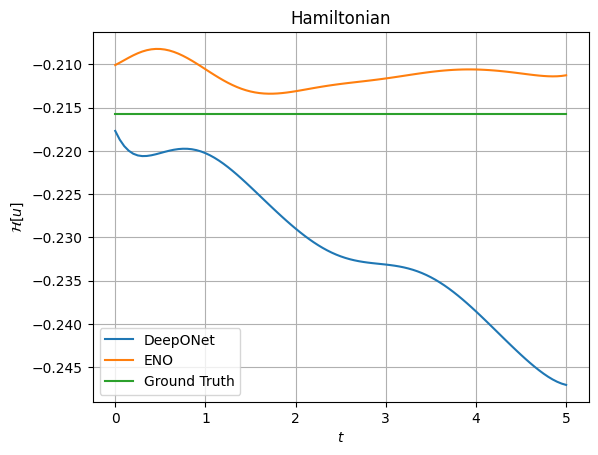
\includegraphics{ENO_Hamiltonian}
    \caption[ENO Hamiltonian]{Just a small test to see if the ENO seems to work. This looks promising to me!}
    \label{fig:ENO_Hamiltonian}
\end{figure}

\begin{table}[h]
    \centering
    \caption{Model Comparison}
    \begin{tabular}{@{}lcccc@{}}
    \toprule
    Model & \# Parameters & Time/Epoch (s) & Epochs Trained & Test Error \\
    \midrule
    DeepONet & 1,234,567 & 12.5 & 100 & 0.05 \\
    FNO & 567,890 & 8.7 & 150 & 0.03 \\
    Modified DeepONet & 1,500,000 & 15.2 & 120 & 0.02 \\ 
    HNO & 987,654 & 10.1 & 200 & 0.04 \\
    HINO & 1,234,567 & 12.5 & 100 & 0.05 \\
    \bottomrule
    \end{tabular}
    \label{tab:model_comparison}
\end{table}

%----------------------------------------------------------------------------------------
%	DISCUSSION
%----------------------------------------------------------------------------------------

%----------------------------------------------------------------------------------------
%	CONCLUSION
%----------------------------------------------------------------------------------------


\appendix % From here onwards, chapters are numbered with letters, as is the appendix convention

\pagelayout{wide} % No margins
\addpart{Appendix}
\pagelayout{margin} % Restore margins

% !TeX root = ..\main.tex
\section*{Github repository}
\addcontentsline{toc}{chapter}{\protect\numberline{}A - Github repository} 

All code files used in this document are included in the Github repository linked below.

\begin{itemize}
    \item \url{https://github.com/eirikfagerbakke/specialization_project}
\end{itemize}

\section*{Notation summary}
\addcontentsline{toc}{chapter}{\protect\numberline{}B - Notation summary}
\begin{table}[h!]
\centering
\begin{tabular}{c|c}
\textbf{Symbol} & \textbf{Description} \\
\hline
\(\mathcal{S}\) & Operator mapping from input to output function space \\
\(\mathcal{A}\) & Input function space (Banach space) \\
\(\mathcal{U}\) & Output function space (Banach space) \\
\(\mathcal{X}\) & Bounded spatial domain \(\subset \mathbb{R}^d\) \\
\(\mathcal{Y}\) & Spatial-temporal domain \(\mathcal{T} \times \mathcal{X} \subset \mathbb{R}^{d+1}\) \\
\(a\) & Input function (initial condition of the PDE) \\
\(u\) & Output function, \(u = \mathcal{S}[a]\) \\
\(y\) & Query point, \(y = (x,t) \in \mathbb{R}^{d+1}\) \\
\(\{a^{(i)}, u^{(i)}\}_{i=1}^N\) & Observations of input-output pairs \\
\(\mu\) & Probability measure supported on \(\mathcal{A}\) \\
\(\mathcal{S}_\theta\) & Neural network approximation of the operator \(\mathcal{S}\) \\
\(\theta\) & Parameters of the neural network \(\in \mathbb{R}^p\) \\
\(\lambda\) & Self-adaptive weights
\end{tabular}
\caption{Summary of notation used in the project.}
\label{tab:notation}
\end{table}


%%%%%%%%%%%%%%%%%%%%%%%%%%%%%%%%%%%%%%%%%%%%%%%%%%%%%%%%


%----------------------------------------------------------------------------------------

\backmatter % Denotes the end of the main document content
\setchapterstyle{plain} % Output plain chapters from this point onwards

%----------------------------------------------------------------------------------------
%	BIBLIOGRAPHY
%----------------------------------------------------------------------------------------

% The bibliography needs to be compiled with biber using your LaTeX editor, or on the command line with 'biber main' from the template directory

\defbibnote{bibnote}{References given in citation order.\par\bigskip} % Prepend this text to the bibliography
\printbibliography[heading=bibintoc, title=Bibliography, prenote=bibnote] % Add the bibliography heading to the ToC, set the title of the bibliography and output the bibliography note

%----------------------------------------------------------------------------------------
%	INDEX
%----------------------------------------------------------------------------------------

% The index needs to be compiled on the command line with 'makeindex main' from the template directory

\printindex % Output the index

\end{document}